% Muster für die Seminarausarbeitung
% HPI Potsdam

\documentclass[11pt, a4paper]{article}

\usepackage{ngerman}
\usepackage[utf8]{inputenc} %Korrekte Kodierung der Umlaute nach UTF-8
\usepackage[T1]{fontenc} %Korrekte Kodierung der Umlaute nach UTF-8
\usepackage{amsfonts}
\usepackage{amssymb}
\usepackage{epsfig}   % Zum Einbinden von Bildern
\usepackage{url}      % Korrekter Satz von URLs
\usepackage{soulutf8}
\usepackage{color}    % Verwendung von Farben
\usepackage{listings} % Korrekter Satz von Listings und Quellcode

%Hilfs-Fonts - ohne Serifen (hier für Tabellen)
\newfont{\bib}{cmss8 scaled 1040}
\newfont{\bibf}{cmssbx8 scaled 1040}

\definecolor{lightgray}{gray}{0.85}

%Seitenformat-Definitionen
\topmargin0mm
\textwidth147mm
\textheight214mm
\evensidemargin5mm
\oddsidemargin5mm
\footskip19mm
\parindent=0in

\begin{document}          

\begin{titlepage}
  \begin{center} 
    \mbox{}
    \vspace{1cm}
    
    {\huge MusicMashup Recommender \\[1em] {\LARGE ein Linked Open Data Musik-Empfehlungsdienst}}  
        
    \vspace{5cm}
    
    Seminararbeit im Seminar \\[1em]
    {\large \sc Linked Data Mashup Programmierung} \\[1em]
    Wintersemester 2014/15 \\[1em]
    Hasso-Plattner-Institut für Softwaresystemtechnik GmbH \\[1em]
    Universität Potsdam
    
    \vspace{4cm}
    
		vorgelegt von
		
    \vspace{1em}
    
        {\Large Dennis Hempfing} \\
		{\Large Paul Wille} \\
		{\Large Karl Wolf}
		
    \vspace{4em}
    
    28.~Februar 2015
  \end{center}
\end{titlepage}


\setcounter{page}{1}

% Zweite Seite = Kurzzusammenfassung
\begin{center}
{\bf Kurzzusammenfassung} 
\end{center}

\noindent
Diese Arbeit gibt einen Einblick in die Funktionsweise des von uns entwickelten Musik-Empfehlungsdienstes MusicMashup, der auf Linked Open Data basiert, und beleuchtet weiterhin die Motivation hinter der Arbeit an diesem System. Im Rahmen des Seminars \glqq Linked Data Mashup Programmierung\grqq bei Dr. Harald Sack (Hasso-Plattner-Institut) haben wir es uns zur Aufgabe gemacht zu zeigen, wie sich unter Nutzung von Linked Data ein vollwertiger Musik-Recommender entwickeln lässt und welche Vor- und Nachteile dadurch entstehen.
Dabei stand neben Linked Data die Fragestellung im Mittelpunkt, wie sich das System im Vergleich zu anderen Musikempfehlungsdiensten abhebt und welchen Mehrwert es dadurch liefert.

\newpage

% Dritte Seite = Inhaltsverzeichnis
\tableofcontents 

\newpage

\section{Einleitung}

Das Internet ist eine Quelle für alle Arten von Daten -- seien es Enzyklopädien wie die Wikipedia oder spezielle Datenbanken für Filme, Bücher, Forschungsergebnisse und viele weitere.


Versucht man nun ein Mashup zu entwickeln, welches verschiedene Datenquellen nutzt, entstehen oftmals Probleme.

\begin{itemize}
\item Die verwendeten Datenquellen verwenden meistens unterschiedliche Formate. Das heißt, dass vor der Verwendung der Daten, diese auf ein gemeinsames Format geführt werden müssen.
\item Auch die Abfrageweise der Daten ist nicht einheitlich. Wird zum Beispiel mit einer SQL-Datenbank und einer API gearbeitet, sind für beide Datenquellen jeweils unterschiedliche Abfrageweise notwendig.
\item Die meisten Datenquellen enthalten keine Verweise auf andere thematisch relevanten Datenquellen. Somit ist ein zusätzliches Maß an Recherche erforderlich, um ausgehend von einer Datenquelle eine weitere zu finden.
\item Viele Datenquellen werden privat verwaltet und sind nicht öffentlich und somit auch nicht frei nutzbar. Solche Datenquellen können nicht verwendet werden und stellen für die Öffentlichkeit keinen Mehrwert dar.
\end{itemize}

Um diese Probleme zu lösen wurde das Prinzip von Linked (Open) Data entwickelt.

\paragraph{} In Kapitel 2 wird zunächst ein kurzer Überblick über die Idee hinter Linked Data gegeben und die Funktionsweise grob skizziert. Darüber hinaus wird die Funktionsweise anderer Musikempfehlungsdienste erklärt und ein Vergleich zu unserem Ansatz gezogen.

\paragraph{} In Kapitel 3 wird der von uns verfolgte Ansatz im Detail erläutert und sowohl von konzeptioneller als auch von technischer Seite beleuchtet.

\paragraph{} In Kapitel 4 kommt es zur Darstellung und Diskussion der erzielten Ergebnisse und es wird auf die Stärken und Schwächen des Systems eingegangen.

\paragraph{} Kapitel 5 ist eine Zusammenfassung der erzielten Ergebnisse und Erkenntnisse. Es folgt ein Ausblick auf mögliche Verbesserungen und Erweiterungen des Systems. 
\newpage
\section{Related Work}


\subsection{Linked Data}

Der Begriff “Linked Data” beschreibt eine Menge an Prinzipien, wie Daten im Internet strukturiert, publiziert und verlinkt werden sollten. Entwickelt worden sind diese von Tim Berners-Lee, der sie 2006 in seinem Bericht “Linked Data” (Q1) veröffentlichte. Die Grundidee dabei ist, sich dafür die Architektur des Internets zunutze zu machen. Im Wesentlichen handelt es sich dabei um vier Punkte:
\begin{enumerate}
\item Verwende zur Bezeichnung von Objekten URIs.
\item Verwende HTTP-URIs, so dass sich die Bezeichnungen nachschlagen lassen.
\item Stelle zweckdienliche Informationen bereit, wenn jemand eine URI nachschlägt (mittels der Standards RDF und SPARQL).
\item Zu diesen Informationen gehören insbesondere Links auf andere URIs, über die weitere Objekte entdeckt werden können.
\end{enumerate}
% (Zitiert nach Q2)

Das erste Prinzip besagt, dass URIs nicht nur benutzt werden sollen, um Dokumente im Internet verfügbar zu machen. Jede Form von Objekten oder Entitäten soll eindeutig über eine URI identifizierbar sein, handele es sich um eine Person, einen spezifischen Gegenstand oder allgemein “Dinge”.


Das zweite Prinzip spezifiert, dass die im ersten Prinzip angesprochenen URIs HTTP-URIs sein sollen. HTTP hat sich im Internet als universales Übertragungsprotokoll etabliert. Die Verwendung von HTTP-URIs ermöglicht es demzufolge, solche URIs einfach nachschlagbar zu machen.


Das dritte Prinzip schlägt die Benutzung eines einheitlichen Formats für die Publikation von Daten vor, in diesem Fall das “Resource Description Framework” (RDF). Dabei handelt es sich um ein simples graphen-basiertes Datenmodell. Bei SPARQL handelt es sich um eine von SQL inspirierte RDF-Anfragesprache.


Das vierte Prinzip plädiert für die Benutzung von Hyperlinks zur Verlinkung einzelner Ressourcen, um den Zugriff auf weitere thematisch relevante Datenquellen zu ermöglichen. Im Gegensatz zu normalen Hyperlinks, welche keinen Kontext beinhalten, lässt sich bei nach RDF spezifizierten Links ein Kontext angeben. So kann zum Beispiel ausgedrückt werden, dass zwei Ressourcen semantisch äquivalent sind oder dass zwei Personen, die miteinander verlinkt werden, befreundet sind.


\subsection{RDF}

Wie bereits beschrieben, handelt es sich bei dem “Resource Description Framework” um ein Graph-basiertes Datenmodell zur Strukturierung von Daten. Die Daten werden dabei in Tripeln organisiert und bilden einen gerichteten Graphen. Ein Tripel besteht aus Subjekt, Prädikat und Objekt und bildet die Struktur eines simplen Satzes ab. Solch ein simpler Satz könnte wie folgt aussehen:

\begin{lstlisting}
 Led Zeppelin (S) ist (P) eine Band (O).
\end{lstlisting}


Das Subjekt eines Tripels ist eine URI, die die Ressource eindeutig identifiziert. Beim Objekt kann es sich um ein Literal, zum Beispiel eine Nummer oder einen String, oder um eine URI handeln, die mit dem Subjekt in Verbindung steht. Das Prädikat spezifiziert in welcher Form Subjekt und Objekt miteinander in Verbindung stehen. Thematisch zusammenhängende Prädikate werden in so genannten Ontologien spezifiziert, wobei auch jedes Prädikat über eine URI dereferenzierbar ist.

Der Satz aus dem obigen Beispiel (“Led Zeppelin” ist vom “Typ” “Band”) wird in der DBPedia folgendermaßen dargestellt:

\begin{lstlisting}
http://dbpedia.org/resource/Led_Zeppelin (S) 
  http://www.w3.org/1999/02/22-rdf-syntax-ns#type (P)
  http://dbpedia.org/ontology/Band (O)
\end{lstlisting}
% (Q3)
Hierbei ist noch zu erwähnen, dass URLs, vor allem solche, die öfter vorkommen, im rdf-Format durch präfixe ersetzt werden können. http://www.w3.org/1999/02/22-rdf-syntax-ns\# wird dann zum Beispiel zum Präfix “rdf:”; Ressourcen aus der DbPedia können durch “dbpedia:” dargestellt werden.
Das genannte Beispiel sieht dann derart aus:

\begin{lstlisting}
dbpedia:Led_Zeppelin (S) rdf:type (P) dbpedia-owl:Band (O)
\end{lstlisting}

In dieser Ausarbeitung werden wir der Lesbarkeit halber ebenfalls gängige Präfixe für Ontologien benutzen. Diese sind:
\begin{itemize}
\item dbpprop: \tt <http://dbpedia.org/property/>
\item dbpedia-owl: \tt <http://dbpedia.org/ontology/>
\item rdf: \tt <http://www.w3.org/1999/02/22-rdf-syntax-ns\#>
\item rdfs:\tt <http://www.w3.org/2000/01/rdf-schema\#>
\item mo: \tt <http://purl.org/ontology/mo/>
\item foaf: \tt <http://xmlns.com/foaf/0.1/>
\item owl: \tt <http://www.w3.org/2002/07/owl\#>
\end{itemize}

\subsection{DBpedia}

Bei der DBpedia handelt es sich um ein offenes Projekt, dessen Ziel es ist, die in der Wikipedia zusammengetragenen Daten nach der RDF Spezifikation zu strukturieren und unter offener Lizenz zu veröffentlichen (Q4). Sie besteht seit 2007 und ist eines der größten Projekte, das sich mit Linked Data befasst. Aufgrund ihrer Größe, des breiten Spektrums an Informationen, welche abgedeckt werden, und der Anzahl der Verlinkungen zu anderen Datensätzen, bildet die DBpedia einen großen Knotenpunkt im Web of Data und ist demzufolge eine gute Grundlage für die Erstellung eines Linked Data Mashups.
% (Q14 Linked Data schaubild als quelle)


\subsection{Existierende Empfehlungsdienste}
\paragraph{} Seitdem Musik gemacht und verkauft wird, besteht auch immer ein Bedarf danach neue Musik zu entdecken, die einem gefällt. Was früher nur durch das Gespräch mit Freunden oder im Plattenladen möglich war, wird heute auch automatisiert im Internet angeboten.

\paragraph{} Man unterscheidet dabei zwischen \textbf{inhaltsbasierten} und kollaborativen Empfehlungsdiensten. (QX-QY: Quellen provided by workaround Karl) Bei ersteren steht die Musik selbst im Mittelpunkt; ausgehend von einem Musikstück oder einer Band wird bestimmt, welche anderen Bands und Liedern diesem ähnlich sind, zum Beispiel durch ein ähnliches Genre oder gemeinsame Mitglieder.

\paragraph{} \textbf{Kollaborative} Empfehlungsdienste dagegen betrachten nicht die Musik als solche, sondern arbeiten mit Statistiken auf Basis der Interaktionen ihrer Nutzer. Ein einfaches Beispiel stellt gnoosic dar, das nach der Eingabe eines Interpreten weitere vorschlägt, für die man jeweils angeben kann, ob man diese ebenfalls mag. 

Der Nutzen dieser Dienste entsteht durch die große Menge an nutzergenerierten Informationen. Durch die Auswertung des Geschmacks vieler Leute lässt sich meist eine präzise Aussage treffen, ob der Hörer von Band A auch Band B schätzt.

\paragraph{} Daneben gibt es auch \textbf{nicht-automatische Varianten} der Musikempfehlung, zum Beispiel durch Freunde, in Musikgeschäften oder Zeitschriften.

\paragraph{} Viele Empfehlungsdienste sind direkt in andere Dienste integriert, so zum Beispiel beim Online-Händler Amazon oder dem Musikstreamingportal Spotify. Diese werten direkt das Kauf- bzw. Hörverhalten ihrer Kunden aus, um damit Empfehlungen zu generieren.  

Außerdem existieren spezialisierte Empfehlungsdienste, so zum Beispiel der BibTip-Service des Karlsruher Instituts für Technologie oder Webseiten wie TasteKid und Musicovery. Wiederum andere Dienste richten sich an spezielle Anwendungszwecke wie Jog.fm, dass je nach Laufgeschwindigkeit die musikalische Untermalung zum Joggen empfiehlt.

Neben den genannten Beispielen lassen sich für jede Kategorie weitere Anbieter finden, auf die jedoch nicht näher eingegangen werden soll.

\paragraph{} Im \textbf{Vergleich} zum vorgestellten Ansatz existieren zwei signifikante Unterschiede. Zum ersten gibt keines der anderen Musikempfehlungssysteme Gründe an, warum bestimmte Interpreten empfohlen werden. Zum zweiten verfolgen die anderen Systeme jeweils einen Ansatz gezielt, haben also zum Beispiel Musik, aber keine Liste anstehender Konzerte oder einen Abstract über den Interpreten, aber keine Möglichkeit Musik abzuspielen. MusicMashup gibt Gründe für die Empfehlungen ab und bietet neben der Empfehlungslogik auch weitere Funktionalität an. Wie dies im Detail geschieht, wird im nächsten Kapitel genauer beschrieben.
\newpage
\section{Aufgabenstellung}


Wir haben uns zum Ziel gesetzt, einen vollwertigen Musikempfehlungsdienst zu entwickeln, welcher auf Basis von Linked Data arbeitet. Inspiriert ist dies durch den Internetdienst Musicbrainz\footnote{\url{http://www.musicbrainz.org/}}. Dabei handelt es sich um eine offene Musik-Enzyklopädie, die zahlreiche Informationen zu Musikern und Bands anbietet. Dazu zählen Informationen wie ein kurzer Abstract, eine Discographie, externe Links, eine Liste aller aktueller und ehemaliger Mitglieder der Band etc. Sucht man auf Musicbrainz zum Beispiel nach der Band \glqq Queens of the Stone Age\grqq, sieht man dort, dass Josh Homme das einzige verbliebene Gründungsmitglied der Band ist. Mit einem Klick auf den Namen wird man zur Seite von Josh Homme weitergeleitet. Dort sieht man unter Anderem in welchen anderen Bands er gespielt hat und kann sich wiederum Informationen zu diesen ansehen.

\paragraph{} Der Benutzer kann also ausgehend von einem Interpreten weitere entdecken. Genau diese Möglichkeit soll auch MusicMashup bieten. Der Benutzer gibt den Names eines Interpreten ein und bekommt passend zu diesem Empfehlungen. Klickt er eine dieser Empfehlungen an, werden ihm wiederum für diesen Interpreten Empfehlungen angezeigt. 


\paragraph{} Erweitert wird dies durch zusätzliche Informationen und Funktionen. Die wohl wichtigste Zusatzfunktion ist ein eingebundener Spotify-Player, welcher die Möglichkeit bietet, sich direkt Musik des jeweiligen Künstlers anzuhören. Darüber hinaus wird eine Liste mit anstehenden Konzerten ausgegeben, sowie weiterführende Links, eine Bildergalerie und ein kurzer Abstract über den Artist. Damit der Benutzer nachvollziehen kann, wie er von einem Interpreten zum Nächsten gekommen ist, wird im Header der Seite eine Liste der zuvor betrachteten Interpreten angezeigt.

\subsection{Technische Grundlagen des Servers}

MusicMashup ist als so genannte Web-App realisiert und präsentiert sich dem Benutzer als interaktive Website, die er aus seinem Browser nutzen kann.

Die programmatische Grundlage von MusicMashup bildet ein in Python geschriebener 
HTTP-Server basierend auf dem \textit{cherrypy}-Modul\footnote{\url{http://www.cherrypy.org/}}. Dieser Server wertet die Nutzeranfrage aus, führt die entsprechenden Abfragen durch und liefert die daraus generierten Empfehlungen mittels der Template-Engine mako\footnote{\cite{http://www.makotemplates.org/}} als Website aus. 

\subsection{Klassenstruktur}


\paragraph{}Das System besteht aus vier Klassen: \textit{MusicMashupServer}, \textit{MusicMashupArtist}, \textit{MusicMashupParser} und \textit{MusicMashupPagerank} (siehe Abb. X).


\begin{figure}[ht!]
\centering
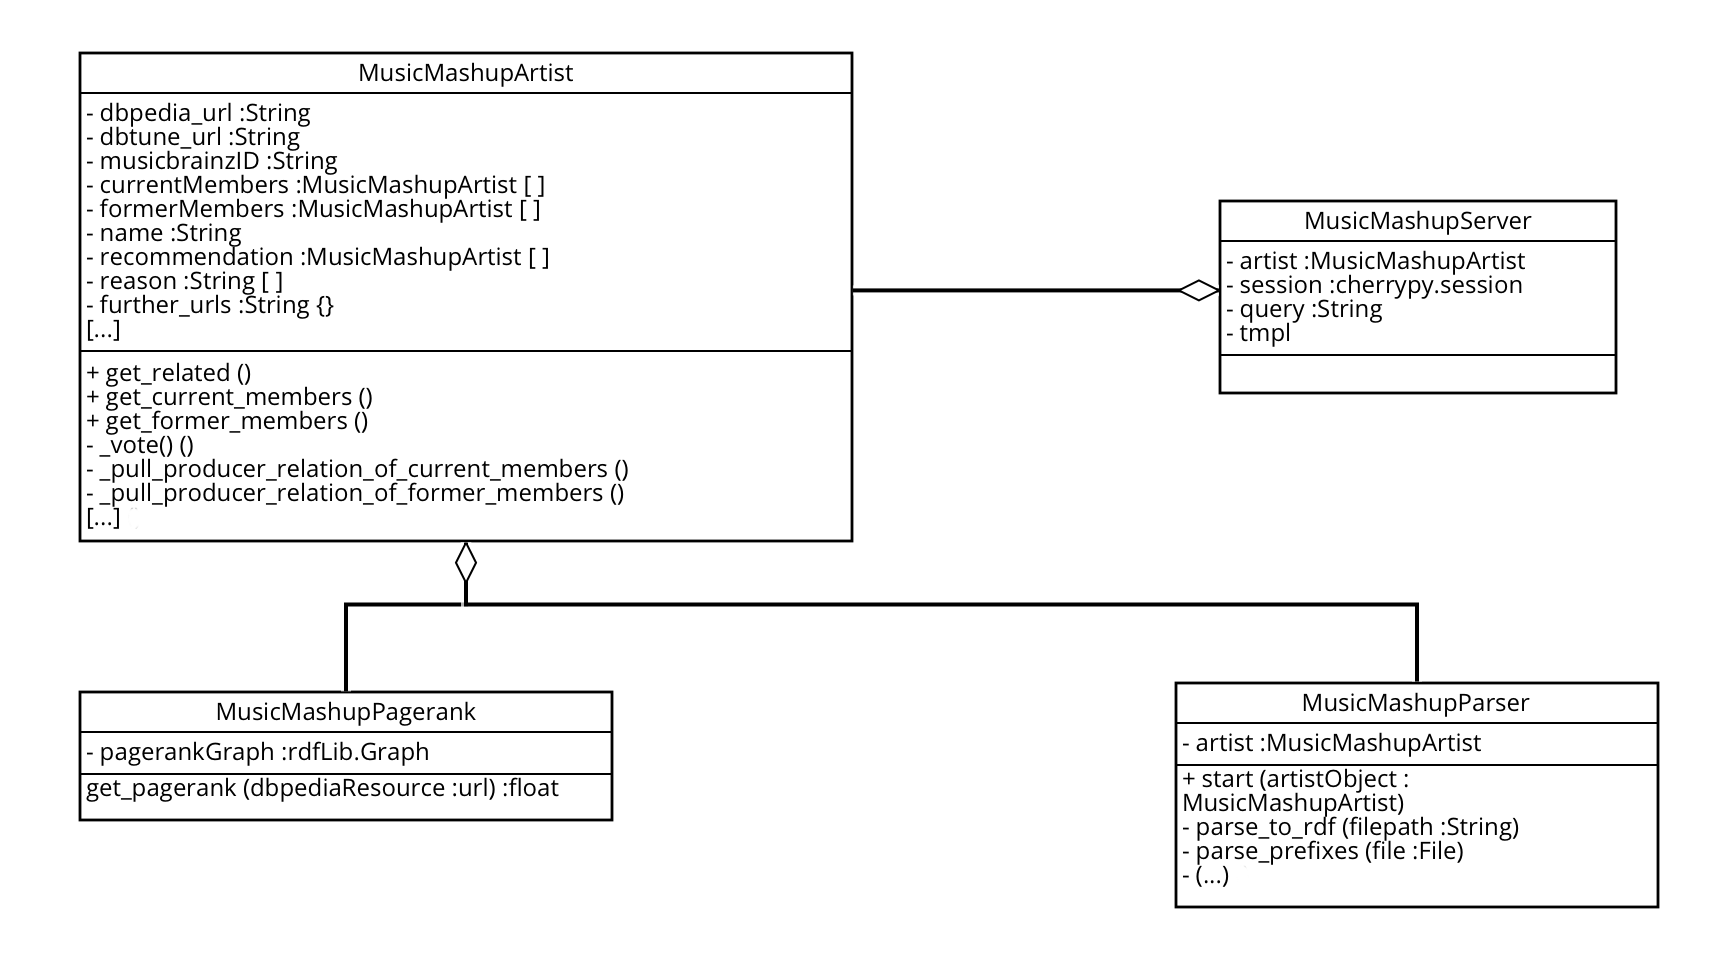
\includegraphics[width=137mm]{bilder/klassendiagramm.png}
\caption{Klassendiagramm der beschriebenen Klassen von MusicMashup \label{overflow}}
\end{figure}

% loest funktionen aus???
\paragraph{Server} Die Klasse \textit{MusicMashupServer} stellt den Web-Server bereit und löst bei einem Aufruf der Anwendung weitere Funktionen aus. Wird nach einem Interpreten gesucht, wird für diesen Interpreten ein Objekt vom Typ MusicMashupArtist erstellt. Diesem wird entweder die Suchanfrage oder aber eine aus einer Empfehlung stammende DBpedia-URL übergeben, sollte eine Empfehlung angeklickt worden sein. Die eigentliche Programmlogik geschieht dann in diesem Objekt. Nachdem diese ausgeführt wurde, wird anschließend das HTML-Dokument gerendert und an den Browser ausgeliefert.


\paragraph{Artist} Die Klasse \textit{MusicMashupArtist} dient als Repräsentation eines Artists. Sie implementiert alle Abfragen, mittels derer Informationen über einen Artist gefunden werden und speichert diese. Darüber hinaus stellt sie Funktionen bereit, die es dem HTML-Template ermöglichen, diese Informationen abzufragen, um sie anschließend anzeigen zu lassen.


\paragraph{Parser} Die Klasse \textit{MusicMashupParser} ist eine simple Implementierung eines Parser, der die Informationen, die zu den Artists gefunden werden, in eine Turtle-Datei (.ttl) schreibt. Bei Turtle handelt es sich um eine Syntax des RDF-Formats, welche eine Repräsentation eines RDF-Graphen in Textform ermöglicht \cite{turtle}. Das Parsen geschieht aus zwei Gründen: erstens liegt nicht jede der Datenquellen in Form von Linked Data vor. Der Parser überführt die Informationen in eine solche Turtle-Datei und ermöglicht so eine Bereitstellung der Daten als Linked Data.  Zweitens kann beim Aufruf eines Artists überprüft werden, ob bereits eine Turtle-Datei existiert, in dem die Informationen zur Verfügung stehen. Falls ja, können diese aus der Datei geladen werden, was zu einer deutlichen Verringerung der Ladezeit führt.


\paragraph{Pagerank} Die Klasse \textit{MusicMashupPagerank} wird einmalig beim Aufruf der Anwendung instanziert und dient als Schnittstelle zum Dump der DBpedia-Pageranks, welche in einen Graphen geladen werden und somit zum Abfragen bereitstehen.

\subsection{Datensätze}

\paragraph{Musicbrainz} Musicbrainz verwendet IDs, um Artists eindeutig zu identifizieren. Diese IDs wurden von vielen anderen Musikdiensten zur Identifikation von Artists übernommen. Um diese zu erhalten, wird eine Anfrage auf DBtune\footnote{\url{http://www.dbtune.org/musicbrainz/}} gestellt. Dabei handelt es sich um ein Linked Data Mapping der Musicbrainz Datenbank. Bei einer erfolgreichen Abfrage erhält das System die Musicbrainz-ID und über \texttt{owl:sameAs} den Link zur entsprechenden DBpedia-Ressource. Da DBtune jedoch nicht vollständig ist (zum Beispiel enthält DBtune keinen Eintrag für die Band \glqq Them Crooked Vultures\grqq), wird als Fallback ein Linked Data Dump der Musicbrainz-Datenbank benutzt. Zwar gibt es in vielen Fällen, in denen es keinen Eintrag auf DBtune gibt, einen Eintrag im Musicbrainz-Dump, jedoch hält der Dump keinen Verweis auf DBpedia, weswegen er schlussendlich nur als Fallback zum Einsatz kommt.

\paragraph{DBpedia} Als Hauptdatenquelle kommt DBpedia zum Einsatz. Von der DBpedia erhält unser System zu einem Interpreten den Abstract, eine Liste der aktuellen und ehemaligen Bandmitglieder sowie ein Thumbnail. Um die bereits vorher genannten zusätzlichen Informationen und Funktionen bereitzustellen, musste auf Datenquellen zurückgegriffen werden, die nicht im Linked Data Format vorliegen. Dazu gehören Spotify für den Musikplayer, Songkick\footnote{\url{http://www.songkick.com/developer/}} für zukünftige Konzerte und Echonest\footnote{\url{http://developer.echonest.com/}}. Echonest dient einerseits als Schnittstelle zu den anderen APIs, andererseits liefert es auch einen sogenannten \glqq Familiarity\grqq-Wert, welcher benutzt wird, um die Relevanz der gefundenen Empfehlungen zu bewerten (dazu später mehr).

\paragraph{Commons} Weiterhin kommen die DBpedia-Commons\footnote{\url{http://commons.dbpedia.org/}} sowie ein Dump der DBpedia-Pageranks \cite{dbpedia-graphmeasures} zum Einsatz. DBpedia-Commons stellt die Wikimedia-Commons als Linked Data bereit. Diese werden benutzt, um zu einer Band Bilder in einer Bildergallerie bereit zu stellen, sollten welche vorliegen. 
Der Dump der DBpedia-Pageranks, welcher von der Semantic-Technologies-Forschungsgruppe des Hasso-Plattner-Instituts bereitgestellt wurde, hält für jede DBpedia-Ressource einen Eintrag über ihren Pagerank. MusicMashup verwendet diesen Dump, reduziert auf Ressourcen mit dem \texttt{rdf:type} \texttt{Band}, \texttt{MusicalArtist} bzw. \texttt{Artist}.

\subsection{Funktionsweise}


Beim erstmaligen Aufruf von MusicMashup wird dem Benutzer eine einfach gestaltete Startseite präsentiert, auf der mittels eines Eingabefelds nach einem Artist  suchen kann, zu dem er sich Empfehlungen geben lassen möchte.


% Bild: Startseite

\subsubsection{Finden von Informationen zum Künstler}
Der vom Benutzer eingegebene Name wird zunächst in Titlecase überführt. Das bedeutet, dass alle Wortanfangsbuchstaben der Eingabe in Großbuchstaben überführt werden, außer es handelt sich um Artikel oder Präpositionen. Wir haben bei unserer Arbeit feststellen können, dass sich somit mehr als 95\% aller Künstler zuverlässig finden lassen.
Anschließend wird auf DBtune nach einer Ressource gesucht, deren \texttt{rdfs:label} mit der Eingabe des Nutzers übereinstimmt und die außerdem als \texttt{rdf:type} den Eintrag \texttt{mo:MusicArtist} hat. Wird eine Ressource gefunden, erhält das System die Musicbrainz-ID des Artists sowie den Link zur DBpedia-Ressource.

Für den Fall, dass sich ein Artist nicht auf DBtune finden lässt, wird im Musicbrainz-Dump nach dem Artist gesucht. Statt \texttt{rdfs:label} kommt hier \texttt{foaf:name} zum Einsatz. Da im Musicbrainz-Dump kein Verweis auf den entsprechenden DBpedia-Eintrag vorhanden ist, muss auf der DBpedia selbst nach der entsprechenden Ressource gesucht werden.

\begin{figure}[ht!]
\centering
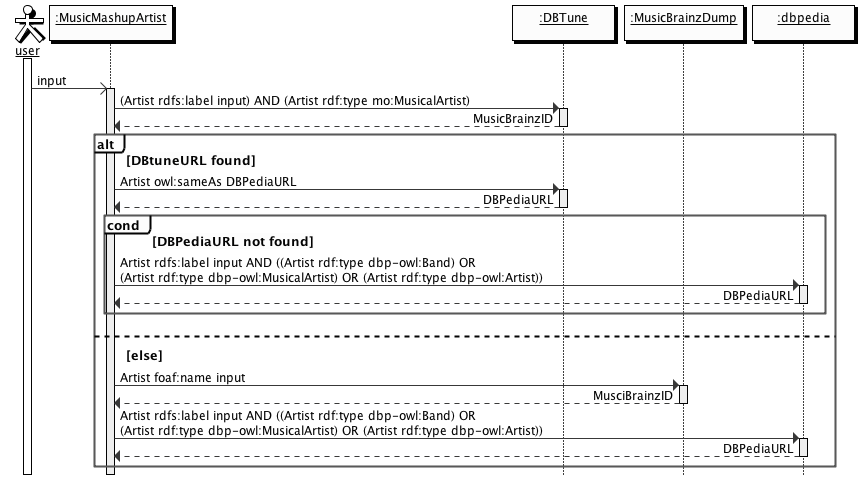
\includegraphics[width=137mm]{bilder/sequenzdiagramm.png}
\caption{Zum gesuchten Künstler wird eine Ressource gefunden \label{overflow}}
\end{figure}


\subsubsection{Suche nach Recommendations}
Ist der Link zur DBpedia-Ressource des jeweiligen Künstlers vorhanden, kann gezielt nach Empfehlungen gesucht werden. Dazu werden zunächst alle aktuellen sowie ehemaligen Mitglieder der Band via \texttt{dbpprop:currentMembers} oder \texttt{dbpedia-owl:bandMembers}  bzw. \texttt{dbpprop:pastMembers} oder \texttt{dbpedia-owl:formerBandMember} abgefragt. Im Anschluss werden für jedes so gefundene Mitglied folgende Relationen überprüft: die Membership-Relation (s.o), die Producer-Relation (\texttt{dbprop:producer} oder \texttt{dbpedia-owl:producer}), die Composer-Relation (\texttt{dbpedia-owl:composer}) und die Writer-Relation (\texttt{dbpedia-owl:writer} oder \texttt{dbpprop:writer}). Grundsätzlich wird für jede Relation nach Bands oder Künstlern gesucht, in denen ein aktuelles oder ehemaliges Mitglied der Band zur Zeit spielt, gespielt hat bzw. nach Bands, für die ein aktuelles oder ehemaliges Mitglied der Band produziert oder einen Song geschrieben bzw. komponiert hat. 

\subsubsection{Auswerten der Empfehlungen}
Wird bei einer dieser Abfragen eine Empfehlung gefunden, gibt es zwei Möglichkeiten: ist der gefundene Artist noch nicht in der Liste der empfohlenen Artists enthalten, wird er der Liste samt des Grundes, warum er empfohlen wird, hinzugefügt. Sollte der gefundene Interpret bereits in der Liste enthalten sein, wird diesem Artist lediglich der Grund hinzugefügt, weshalb er gefunden wurde.  % vllt umbauen?


Nachdem alle Relationen überprüft wurden, wird mittels eines Voting-Algorithmus über die Relevanz der einzelnen Empfehlungen entschieden. Dafür wird der Familiarity-Wert genutzt, den die Echonest-API bereit stellt, sowie die DBpedia-Pageranks. Die Echonest-Familiarity ist ein von Echonest errechneter Wert, der aussagt, wie bekannt die Band ist.\cite{echonest_familiarity}
% anhand? bekannt ggf. ersetzen?

\paragraph{} Des weiteren wird jeder Relation ein Faktor zugeordnet, der mit in die Berechnung einfließt. Diese Faktoren haben die Aufgabe, die Wichtigkeit der Relationen untereinander zu bewerten. Die Membership-Relation für aktuelle Bands hat den höchsten Faktor, gefolgt von der Membership-Relation für ehemalige Bands, der Producer-Relation und der Writer- und der Composer-Relation, welche gleichwertig sind. Geht diese Relation von einem aktuellen Mitglied der Band aus, so ist der Faktor doppelt so hoch wie für ein ehemaliges Mitglied. Am Ende werden der DBpedia-Pagerank, die Echonest-Familiarity und der Relationsfaktor miteinander multipliziert. Die Empfehlung mit dem höchsten Wert steht in der Liste der Vorschläge oben und die mit dem niedrigsten Wert unten.
Nach Abschluss des Votings wird der Parser gestartet, welcher alle gefundenen Informationen für einen Artist in eine Turtle-Datei schreibt. % ehemalige band? 2x am Ende

\paragraph{} Wurden alle Schritte erledigt, kann die Seite gerendert und ausgegeben werden (siehe Abb. x).


% Bild einer fertigen Seite
\newpage
Diskussion der erzielten Ergebnisse


Durch den im vorherigen Absatz beschriebenen Ansatz ist es gelungen, mit dem MusicMashup-Recommender einen vollwertigen Recommender-Dienst vorweisen zu können. Da es im Internet einige Music-Recommender-Dienste gibt (vgl. das Kapitel Related Work), stellt sich die Frage, inwiefern sich dieses Produkt von anderen abhebt. Zumal neben dedizierten Empfehlungsdiensten auch viele andere Dienste (Spotify, Grooveshark, Youtube, Amazon u.v.m.)  eine Empfehlungslogik eingebaut haben.
Ein wichtiges, wenn nicht das wichtigste Alleinstellungsmerkmal, ist der Ansatz, eine Nachvollziehbarkeit für den Nutzer, aus welchen Gründen Empfehlungen zu einem Interpret gefunden wurden, bereitzustellen. Dies kann außer durch manuelle Suche in großen Musikdatenbanken wie beispielsweise discogs so nicht mit anderen Recommendation-Diensten erreicht werden.
Im Falle von Musik zielen Recommendation-Dienste meistens darauf ab, dem Nutzer “ähnliche” Musik vorzuschlagen und ihm dadurch zu zeigen, welche Interpreten zu dem gesuchten Interpret oft in Verbindung gebracht werden, beziehungsweise bei welchen Interpreten sich die Geschmäcker einer Vielzahl von Hörern überschneiden.
Der Ansatz des MusicMashup-Recommenders ist da deutlich pragmatischer, da direkte Verknüpfungen der Mitglieder einer Band oder eines Solo-Artisten als Grund dienen, einen Interpreten vorzuschlagen.
Das Ziel ist es aber auch, mit dem MusicMashup-Recommender eine Zielgruppe zu erreichen, die eher als musikaffin zu bezeichnen ist und sich für die Hintergründe interessiert und nicht einfach nur neue ähnliche Musik entdecken will. Deshalb wurde bei der Entwicklung darauf Wert gelegt, dem Nutzer die Gründe für einen Vorschlag gut sichtbar und verständlich anzuzeigen.


Neben der Art der Vorschläge ist ein weiterer Ansatz [g]des MusicMashup-Recommenders, die Bedienung so dynamisch[h][i] wie möglich zu gestalten. So ist es möglich, auf alle vorgeschlagenen Interpreten aber auch Bandmitglieder zu klicken, um wiederum Vorschläge für diesen Interpreten zu erhalten. Es werden also nicht nur für eine getätigte Eingabe Empfehlungen ausgegeben, sondern man erlangt durch Anklicken eben dieser Empfehlungen erneut Informationen zu diesen. Dies soll den Nutzer dazu einladen, unbekannte Zusammenhänge zu entdecken und das Wirken von Bands oder Solokünstlern, die ihn interessieren anhand von Gründen nachzuvollziehen. Durch die prominent platzierte Anzeige eines Pfades, der Breadcrumb-ähnlich dargestellt wird, soll ermöglicht werden, dass der Nutzer auch nach längerem Entdecken noch die Möglichkeit hat, nachzuvollziehen, wie er zu dem aktuellen Interpreten gelangt ist und gegebenenfalls zu einem Artist des Pfades zurückspringen kann, sollte er sich nicht weiter in die eingeschlagene Richtung vertiefen wollen.
 breadcrumbs.png 

Da dieses Produkt sich mit Musik beschäftigt, stand der Anspruch immer im Vordergrund, dem Nutzer direkt das Hören der Musik eines Interpreten zu ermöglichen. Nach längerer Evaluation viel die Wahl auf Spotify als Anbieter. Dies schränkt zwar die Zielgruppe ein, da ein Account erforderlich ist, allerdings ist Spotify einer, wenn nicht der etablierte Musikdienst zum kostenlosen Musikhören. Außerdem bietet Spotify zu fast jedem Künstler eine große Auswahl an Musik. Entscheidend für die Wahl von Spotify war vor allen Dingen auch, dass es trotz einfacher Einbindung in die UI einen vom Browser entkoppelten Weg ermöglicht, Musik abzuspielen. Dies bietet den entscheidenden Vorteil, dass Musik im Hintegrund weiterläuft, auch wenn im Browser neue Künstler angeklickt werden. Eine solche Verknüpfung des tatsächliche Hörens von vorgeschlagenen Künstlerns im Zusammenspiel mit der ständigen Möglichkeit parallel dazu weitere Relationen zu entdecken, ist in einer solchen Form schwer zu finden.


Zusätzlich zu den Vorschlägen, der Bedienung und der ständigen Möglichkeit, die Künstler auch anzuhören, zeichnet sich der MusicMashup-Recommender dadurch aus, dass er dem Nutzer Zusätzliche Informationen übermittelt, die interessant sind, sobald er sich zu einem Artisten genauer informieren will. Eine Liste der aktuellen und ehemaligen Bandmitglieder, welche auch einzeln anklickbar sind, sodass das System gleichermaßen für Bands, wie auch für Bandmitglieder und Solokünstler funktioniert, findet man bei anderen Music-Recommendern selten in dieser Art, was MusicMashup durchaus von anderen Empfehlungsdiensten abhebt. 
Neben dem in fast allen Diensten angezeigten Abstract hat der Nutzer mit dem MusicMashup-Recommender die Möglichkeit bei Bedarf durch Links zu anderen Musikrelatierten Diensten weitere Informationen über den Interpret zu erlangen. Dabei werden (jeweils wenn vorhanden) neben der Wikipedia, der offiziellen Website eines Künstlers und dem www.myspace.com-Profil sowohl www.discogs.com (sehr genau gepflegte Datenbank über Diskographien von Musikern), als auch www.last.fm als weiterer Recommender verlinkt. Für Songtexte steht ein Link zu www.musixmatch.com bereit. Außerdem wird das www.twitter.com Profil verlinkt. Um einen Überblick über aktuelle Live-Events zu gewähren, werden außerdem noch anstehende Konzerte direkt in der UI angezeigt, die jeweils einen Link auf www.songkick.com enthalten.


Insgesamt stehen dem Nutzer so viele Möglichkeiten und weitere Schritte zur Verfügung, einen Künstler zu ergründen. Im Gegensatz zu dem eher statischen Ausliefern an Vorschlägen und der Möglichkeit einzelne Lieder anzuhören, bietet MusicMashup-Recommender eher den Reiz, weiter auf dieser Plattform Musik zu erkunden, anstatt nach einmaliger Info zu einem Künstler zufrieden zu sein. Durch die Entkopplung von Musik und Browser ist auch ein Weitererkunden möglich, während die Musik weiterläuft.


Einer der Aspekte, die sicherlich noch großes Verbesserungspotential bergen, ist der Voting-Algorithmus und die teilweise fehlende Aussagekraft einer vorgeschlagenen Relation. Auf Grund der großen Variationen an Vorschlägen (wenige bzw. gar keine bis hin zu über 100 (z.B. Bob Dylan)) und einer tewilweise zufälllig wirkenden Anordnung bedarf der Voting-Algorithmus einer Überarbeitung beziehungsweise Ergänzung. Die Pageranks aus der dbpedia und der familiarity-Wert der Echonest-API dienen zwar in der Theorie als guter Indikator für die Bekanntheit eines Interpreten, allerdings kann dies auch eine verwirrende Wirkung haben, wenn ein Interpret mit einer eigentlich unwichtigen Begründung[j][k] durch seine Bekanntheit nahezu immer oben gelistet wird. Eine erneute Evaluation der Werte, die für einen gefundenen Grund berechnet werden, wird hier von Nöten sein. Es ist schwierig, einen ausgewogenen, generischen Voting-Algorithmus von Beginn an vorweisen zu können, da dieser viel getestet und angepasst werden muss und einige edge-cases erst nach einiger Zeit auffallen.


Neben der teilweise ungenauen Bewertung der Gründe gibt es auch noch semantisches Ergänzungspotential, welches in Zukunft noch implementiert werden wird. So sollten zum Beispiel Artisten, die zwar mehrere Begründungen enthalten, die aber alle von der gleichen Person stammen, weniger zählen, als Bands, bei denen diese alle von unterschiedlichen Personen stammen. Dies erfordert allerdings eine Neuimplementierung der Datenstruktur der  Begründungen (diese werden derzeit nur als Strings in Textform abgespeichert), um dies generisch zu ermöglichen und war bis zum jetzigen Zeitpunkt noch nicht möglich.


Ein Nachteil gegenüber anderen Music-Recommender-Diensten ist außerdem, dass bei Interpreten, deren Mitglieder oder welche selbst nicht noch anderweitig tätig waren, gar keine Vorschläge gefunden werden können. Hier wäre es denkbar, stattdessen Related-Artists anzuzeigen, die zum Beispiel Spotify oder Echonest über ihre API liefern, oder die dbpedia selbst als associatedMusicalArtist listet. Allerdings würde dies dem eigentlichen Ansatz widersprechen, nur aus klar erkennbaren Gründen Bands vorzuschlagen. Sollte diese Lösung trotzdem Anwendung finden, um zu verhindern, dass man an einem toten Ende des Recommenders anlangen kann, so müsste dies allerdings erkenntlich gemacht werden.


Ein weiterer Punkt, welcher den MusicMashup-Recommender zusätzlich mit am meisten einschränkt, ist die Unvollständigkeit gerade bei unbekannteren oder neueren Musikern. Da als Musikdatenquelle ein nur eingeschränkt vollständiges Mapping der an sich umfangreichen Musikatenbank musicbrainz dient, welches durch ein Fallback mit einem weiteren Dump ergänzt wird, welches Wiederum eine Verlinkung zur dbpedia vermissen lässt, kommt es oft zu leeren Seiten. Für einige Fälle konnte hier eine Lösung gefunden werden, trotzdem Ergebnisse zu liefern, allerdings gab es leider keine generische.
Das ist eine sehr große Einschränkung der Nutzbarkeit. Die Abhängigkeit von der Vollständigkeit und Genauigkeit der benutzten Datensätze wird hier sehr gut deutlich. Neben vielen Vorteilen, die das Benutzen von Linked Open Data mit sich bringt, zeigt sich hier, dass es sehr wünschenswert wäre, wenn weitere Datenbanken zu kompletten Themengebieten - wie zum Beispiel Musik - in Linked Data vorliegen würden.


Generell allerdings hat das Benutzen von Linked-Data-Quellen und dem Folgen des Linked Data Ansatzes den großen Vorteil, dass die Daten bereits von Anfang an standardisiert, maschinenlesbar kodiert und verlinkt sind.


So ist das Zusammenführen der Arten simpel und die Programmierung nicht davon abhängig, für jede verwendete API die Daten selbst in das gewünschte Format zu überführen. Auch der Kontext muss nicht manuell und fehleranfällig selbst hergestellt werden, etwa durch Suchen, sondern war von vornherein bekannt. Hierdurch konnte der Fokus bei der Programmierung von Anfang an auf die Arbeit mit den Daten gelegt werden. Bei der Verwendung anderer Quellen hätte man diese zunächst noch verarbeiten und selbst standardisieren müssen, um überhaupt mit ihnen umgehen zu können.


Auch der Fakt, dass es sich bei Linked-Data-Datenquellen um  offene Datenquellen handelt, hat die Arbeit wesentlich erleichtert und beschleunigt, da keine Schlüssel oder ähnliches für die Verwendung proprietärer APIs beschafft und implementiert werden mussten. 


Als hilfreich stellte sich auch heraus, dass für RDF und SPARQL bereits Bibliotheken existierten, auf die bei der Programmierung zurückgegriffen werden konnte.


Besonders hilfreich war, dass die Verlinkung zwischen einzelnen Ressourcen jeweils in einem Kontext standen. Dies machte es einfach, für die ausgegebenen Empfehlungen einen Kontext zu liefern, was ein Kernkonzept von MusicMashup ist.[l][m][n]
\newpage
\section{Zusammenfassung}

Diese Arbeit hat einen Einblick in die Funktionsweise von MusicMashup-Recommender gegeben und ist auf Vor- und Nachteile von Linked Data im Rahmen des Projekts eingegangen. Das Ergebnis des Projekts ist ein vollwertiges, wenn auch erweiterbarer MusicRecommendationSystem, mittels welchem Benutzer sich Empfehlungen für neue Artists geben lassen können. Zusätzlich dazu werden ein Musikplayer, eine Liste anstehender Konzerte und weitere Informationen angeboten. Die so gesammelten Informationen werden mittels eines Parsers als Linked Data abgespeichert und können veröffentlich werden.




%Hier kommt das Literaturverzeichnis
\newpage

\addcontentsline{toc}{section}{Literaturverzeichnis} % Zeile für das Inhaltsverzeichnis
\nocite{*}
\bibliography{references}
\bibliographystyle{alphadin}


\end{document}
